% 8185: Quant Bhandari PS3

\documentclass[12pt]{article}
%\usepackage[T1]{fontenc}
%\usepackage{lipsum}
\renewcommand{\baselinestretch}{1.2} 
\usepackage{graphicx}
\usepackage{hyperref}
\hypersetup{
    colorlinks=true,
    urlcolor=blue,
    citecolor=blue
}
\usepackage[export]{adjustbox}
\usepackage{subcaption}
\usepackage{amsmath}
\usepackage{amssymb}
\usepackage{amsfonts}
\usepackage{geometry}
\setcounter{MaxMatrixCols}{20}
\geometry{a4paper,
 left=3cm,right=3cm,
 top=1.5cm, bottom=1.5cm}

\usepackage{natbib}
\bibliographystyle{apalike}


%\usepackage{natbib}
%\setcitestyle{authoryear,open={(},close={)}}
\graphicspath{ {../figs/} }

\begin{document}
%\thispagestyle{myheadings}
%\markright{Indian Statistical Institute, New Delhi\hfill }

\title{Notes on Aiyagari using EGM}
\author{Bipul Verma}
\date{\today}
\maketitle

%\tableofcontents{}
\abstract{This document calculates the Policy rules for Aiyagari Model using Endogenous grid method.}

\vspace{8cm}

%\begin{center}
%\includegraphics[scale=0.4]{isi_logo.png}
%\end{center}
%\begin{center}
%\begin{Large}
%INDIAN STATISTICAL INSTITUTE, NEW-DELHI.
%\end{Large}
%\end{center}


\newpage

\section{Basic Aiyagari Model}
We'll start with the basic Aiyagari model first with no endogenous labor, taxes, transfers or government. The basic Aiyagari model has the households solving the following optimization problem:
\begin{align*}
\max_{c_{it}} \mathbb{E}_0 \sum_{t=0}^{\infty} \beta^t \frac{c_{it}^{1-\gamma}}{1-\gamma} \\
\text{s. t.  } c_t + a_{t+1} = w_t\epsilon_t + (1+r_t)a_t \\
a_{t+1} \geq 0.
\end{align*}
The household optimization problem can be summarized in the following Euler condition:
\begin{align*}
u_c(c(a, \epsilon)) & \geq \beta (1+r) \sum \Pi(\epsilon'|\epsilon)u_c(c(a'(a, \epsilon), \epsilon') \\
 & (= \; \text{ if } \; a'(a, \epsilon) >0).
\end{align*}
For the purpose of present exercise we'll also assume that the shocks follow a Markov process with transition matrix $\Pi$.

\subsection{Computation Algorithm: Policy Function}
\begin{enumerate}
\item We need to compute the consumption policy function $c(a, \epsilon)$. We can always use the budget equation to back out the asset policy function.  
\item Construct grid for assets ($a$) and  labour supply shocks ($\epsilon$).
\item Guess the policy function as $c^{(m)}[a_i, \epsilon_j] = ra_i + \epsilon_j$.
\item We'll now calculate the current current consumption and asset levels for a given target level of assets tomorrow.
\item Compute $c^*[a'_i, \epsilon_j] = Uc^{-1}(\beta(1+r)\sum \Pi(\epsilon'|\epsilon_j)u_c(c^{(m)}(a'_i, \epsilon'))$.
\item Compute $a^*[a'_i, \epsilon_j] = (c^*[a'_i, \epsilon_j] + a'_i -w\epsilon_j)/(1+r).$
\item We thus have the policy function $c^*$ defined on endogenous grid of assets $a^*$. We'll interpolate the policy function such that it is defined on the original asset grid.
\item Update as follows:
\begin{align*}
c^{(m+1)}[a_i, \epsilon_j]= 
\begin{cases}
(1+r)a_i + w\epsilon_j - a_0 & \; \; ;  a_i < a^*[a_0, \epsilon_j] \\
\text{LinearInterpolate} (c^*[a_k, \epsilon_j], c^*[a_{k+1}, \epsilon_j])  & \; \; ; a^*[a_k, \epsilon_j] < a_i < a^*[a_{k+1}, \epsilon_j] \\
\end{cases}
\end{align*}
\item Repeat till convergence.
\item \textit{Check at this point of time that the asset policy function for the lowest shock is below the 45 degree line.}
\end{enumerate}

\subsection{Computation Algorithm: Stationary Distribution}
Note that the distribution in the present case is defined over the continuum $(a, \epsilon)$. We can discretize the space and keep track of distribution by assigning densities to those discrete points. These densities will then evolve according to transition matrix based on the asset policy function. Note that one needs to be careful on what transition probabilities each entry of transition matrix $Q$ represents. We'll take a short detour to make the matter more concrete. Suppose that we have a first order markov process $s$ which can take value $\{H, L\}$ with the associated transition matrix $T$ given by:
\begin{align*}
\begin{bmatrix}
\pi(L|L) & \pi(H|L) \\ \pi(L|H) & \pi(H|H)
\end{bmatrix}
\end{align*}
where $\pi(s'|s)$ represents the probability of moving from state $s$ to $s'$. In this case the probability over states evolves according to:
\begin{align*}
\lambda(s') = T' \lambda(s).
\end{align*}
The following code constructs a transition matrix and looks for the stationary distribution. Note that in our case matrix $Q$ is like $T'$ in the previous case.
\subsubsection*{Construction of Q'}
The idea of construction of $Q'$ is the following. For agent at each state today $(a, \epsilon)$, we first find out the asset level that the agent will end up next tomorrow based on the policy function. We then combine this with all possible realization of income shock that the agent can receive in the next period, based on the markov process for $\epsilon$. Below is the algorithm which implements this.
\begin{itemize}
\item For each $\epsilon_j$;
\item $s_j = (j-1)*N_a$
    \begin{itemize}
       \item  for each $a_i$;
       \item find $k$ s.t $a_k \leq a'(a_i, \epsilon_j) < a_{k+1}$,
       \item  construct the histogram weights as $w_k = \frac{a'(a_i, \epsilon_j) - a_k}{a_{k+1} - a_k}$;
       \begin{itemize}
        \item for each $\epsilon_m$;
        \item $t_m = (m-1)*N_a$,
        \item \begin{align*}
          Q'[i+s_j,k+t_m ] & = (1-w_k)\pi(\epsilon_m|\epsilon_j) \\
          Q'[i+s_j,k+1+t_m] & = w_k \pi(\epsilon_m|\epsilon_j) .
        \end{align*}
       \end{itemize}
    \end{itemize}
\end{itemize}

\subsubsection*{Construction of Q}
\href{https://alisdairmckay.com/Notes/HetAgents/Aiyagari.html}{McKay(2018)} outlines the construction of $Q$ directly. The idea is simply to interchange the rows and columns in the last step, i.e
\begin{align*}
          Q[k+t_m, i+s_j ] & = (1-w_k)\pi(\epsilon_m|\epsilon_j) \\
          Q[k+1+t_m, i+s_j] & = w_k \pi(\epsilon_m|\epsilon_j) .
\end{align*}

\subsection{Equilibrium r and w}
Once we have the stationary distribution of individuals over the states, we can calculate the equilibrium interest rate which clears the market. Let $\bar{\mu}$ denote the stationary distribution over $(a, \epsilon)$. Then the aggregates are given by:
\begin{align*}
C & = \int c(a, \epsilon)d\bar{\mu}(a, \epsilon) \\
K & = \int a'(a, \epsilon)d\bar{\mu}(a, \epsilon) \\
N & = \int \epsilon d\bar{\mu}(a, \epsilon)
\end{align*}

Note that at the stationary distribution we'll have $K' = \int a'(a, \epsilon)d\bar{\mu}(a, \epsilon) =  K = \int a d\bar{\mu}(a, \epsilon)$. Hence the aggregate resource constraint will be given by:
\begin{align*}
C + \delta K =  K^{\theta}N^{1-\theta} 
\end{align*}

In order to compute the equilibrium $r$, we find $r$ such that $K^d = K^s$, where:
\begin{align*}
K^d(r) & = N(\frac{r+\delta}{\theta})^{\frac{-1}{1-\theta}} \\
K^s(r) & = \int a'(a, \epsilon; r)d\bar{\mu}(a, \epsilon; r) 
\end{align*}

Finally, to get the distribution of assets across the agents, we make use of the stationary distribution of agents across states to compute the proportion of agents at various assets levels.

\subsection{Results from Basic Aiyagari}
\begin{figure}[h]
    \centering
    \begin{minipage}{0.45\textwidth}
        \centering
        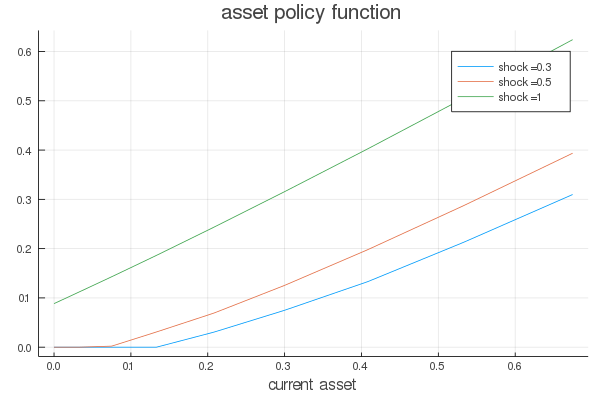
\includegraphics[width=1\textwidth]{A_p_basic.png} % first figure itself
        \caption{Asset Policy Function}
    \end{minipage}\hfill
    \begin{minipage}{0.45\textwidth}
        \centering
        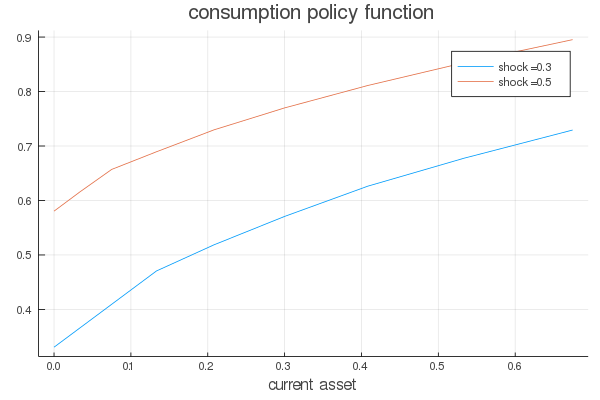
\includegraphics[width=1\textwidth]{C_basic.png} % second figure itself
        \caption{Consumption Policy function}
    \end{minipage}
\end{figure}

\begin{figure}[h]
    \centering
    \begin{minipage}{0.45\textwidth}
        \centering
        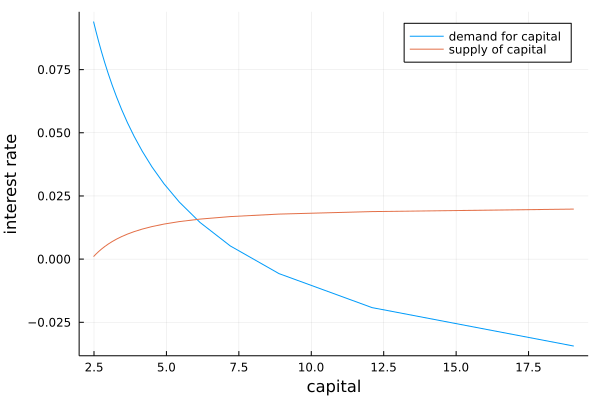
\includegraphics[width=1\textwidth]{basic_aiya_r.png} % first figure itself
        \caption{Asset Market Clearing}
    \end{minipage}\hfill
    \begin{minipage}{0.45\textwidth}
        \centering
        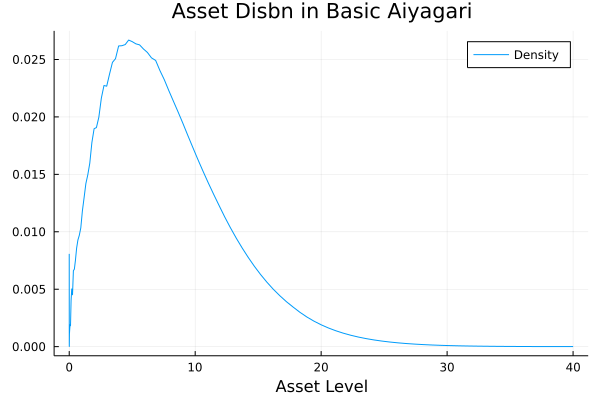
\includegraphics[width=1\textwidth]{basic_aiya_A_dis.png} % second figure itself
        \caption{Stationary Disbn of Assets}
    \end{minipage}
\end{figure}

%% References
%1. http://pages.stern.nyu.edu/~dbackus/Computation/Violante%20endogenous%20grid.pdf
%2. https://www.cemfi.es/~pijoan/download/notes-on-endogenous-grid-method.pdf

\newpage
\section{Aiyagari with Endogenous Labor}
The Aiyagari model with endogenous labor is can be written as:
\begin{align*}
\max \mathbb{E}_0 \sum \beta^t U(c_t, l_t) \\
\text{s.t.  } \;\;\; c_t + a_{t+1} = (1+r)a_t + w_t \epsilon_t (1-l_t) \\
a_{t+1} \geq 0\\
\end{align*}

The consumers optimization is summarized by the following conditions:
\begin{align*}
U_c(c, l) & \geq \beta(1+r) \mathbb{E} U_c(c', l')\\
&(= ) \text{if  } a' >0 \\
\frac{U_l(c, l)}{U_c(c, l)} & = w \epsilon
\end{align*}


\subsection{With separable utility}
In this case the utility function is assumed to be of the following form:
\begin{align*}
U(c, l) = \frac{c^{1-\mu} -1}{1-\mu} - \psi \frac{(1-l)^{1+\frac{1}{\gamma}}}{1+ \frac{1}{\gamma}}.
\end{align*}
For this utility function, the expression for marginal utility are:
\begin{align*}
U_c(c, l) = c^{-\mu} \\
U_l(c, l) = \psi (1-l)^{\frac{1}{\gamma}}
\end{align*}
The consumers consumption leisure choice tradeoff at optimum can then be summarized as follows:
\begin{align*}
\frac{\psi(1-l)^{\frac{1}{\gamma}}}{c^{-\mu}}  = w\epsilon 
\end{align*}
We can thus solve for labor choice in terms of consumption choice at the optimum:
\begin{align*}
l(c) = 1- [\frac{w \epsilon c^{-\mu}}{\psi}]^{\gamma}.
\end{align*}
In this case the with can use the EGM to solve for consumption policy function and solve labor as residual given consumption using the MRS. The only additional modification will be in the update equation for consumption policy where we need to use root finding to solve for implicit $c^{j+1}$, when the asset constraint binds.  In this case the update equation is given as follows:
\begin{align*}
c^{(m+1)}[a_i, \epsilon_j]= 
\begin{cases}
(1+r)a_i + w\epsilon_j(1-l(c^{(m+1)}[a_i, \epsilon_j])) - a_0 & \; \; ;  a_i < a^*[a_0, \epsilon_j] \\
\text{LinearInterpolate} (c^*[a_k, \epsilon_j], c^*[a_{k+1}, \epsilon_j])  & \; \; ; a^*[a_k, \epsilon_j] < a_i < a^*[a_{k+1}, \epsilon_j] \\
\end{cases}
\end{align*}
\textbf{Note:} When the asset constraint is binding, we need to use a root solver to find $c^*$. A trick to improve the speed of EGM iteration comes from noticing the fact that when the asset constraint in binding, we are solving the same set of equations. Hence all these roots can be evaluated outside the iteration loop, rather than each time during the iteration.

\subsection{Without separable utility}
Consider the utility function as given below:
\begin{align*}
U(c, l) = \frac{(c^\eta l^{1-\eta})^{1-\mu}}{1-\mu}.
\end{align*}
For this utility function, the expression for marginal utility are:
\begin{align*}
U_c(c, l) = (c^\eta l^{1-\eta})^{-\mu} \eta (\frac{c}{l})^{\eta -1} \\
U_l(c, l) = (c^\eta l^{1-\eta})^{-\mu} (1-\eta) (\frac{c}{l})^{\eta}
\end{align*}
The consumers consumption leisure choice tradeoff at optimum can then be summarized as follows:
\begin{align*}
\frac{1-\eta}{\eta}\frac{c}{l}  = w\epsilon 
\end{align*}
We can thus solve for labor choice in terms of consumption choice at the optimum:
\begin{align*}
l(c) = \frac{1-\eta}{\eta}\frac{c}{w\epsilon }
\end{align*}


\subsection{Computation Algorithm}
\begin{enumerate}
\item Guess policy function for consumption $c^j(a_i, \epsilon_j) = ra_i + w \epsilon_j$.
\item For this guess of $c^j$ solve the $c^*$ such that the following euler holds on future assets:
\begin{align*}
U_c(c^*(a_i', \epsilon_j), l(c^*(a_i', \epsilon_j))) = \beta(1+r) \sum \Pi(\epsilon'|\epsilon_j) U_c(c^{(j)}(a_i', \epsilon'), l(c^{(j)}(a_i', \epsilon')))
\end{align*}
Note that given the form of utility function the expression for $U_c(c, l(c))$ can be simplified as follows:
\begin{align*}
 \text{When  } l(c) < 1\\ 
U_c(c, l(c)) & =  (c^\eta l(c)^{1-\eta})^{-\mu} \eta (\frac{c}{l(c)})^{\eta -1} \\
 & = (c^\eta (\frac{1-\eta}{\eta}\frac{c}{w\epsilon })^{1-\eta})^{-\mu} \eta (\frac{c}{(\frac{1-\eta}{\eta}\frac{c}{w\epsilon })})^{\eta -1} \\
 & = c^{-\mu} (\frac{1-\eta}{\eta}\frac{1}{w\epsilon })^{(\eta-1)\mu} \eta (\frac{1-\eta}{\eta}\frac{1}{w\epsilon })^{1-\eta} \\
 & = \eta c^{-\mu} (\frac{1-\eta}{\eta}\frac{1}{w\epsilon })^{(1-\eta)(1-\mu)}\\
 & = c^{-\mu} \Phi(\epsilon) \; \; \; \; \; \text{where  } \Phi(\epsilon)  = \eta (\frac{1-\eta}{\eta}\frac{1}{w\epsilon })^{(1-\eta)(1-\mu)};\\
 \text{When  } l(c) = 1\\ 
 U_c(c, l(c)) & = \eta c^{\eta(1-\mu)-1}.
\end{align*}
Note that $U(c, l(c))$ is continuous and monotonically decreasing in $c$. Hence $U_c^{-1}(.)$ is well defined. We need to solve for $c^*$ which solves the following:
\begin{align*}
U_c(c^*(a_i', \epsilon_j), l(c^*(a_i', \epsilon_j))) = \beta(1+r) \sum \Pi(\epsilon'|\epsilon_j) U_c(c^{(j)}(a_i', \epsilon'), l(c^{(j)}(a_i', \epsilon'))).
\end{align*}
One way to solve for $c^*$ is to simply use a root finding algorithm. However, root finding can be time intensive. We can use the following analytical approach to get $c^*$. Compute $c^*_1, c^*_2$ from the analytical expression for two pieces of $U_c$. Compute $l(c^*_1), l(c^*_2)$. If $l(c_1^*) <1$, then $c^* = c^*_1$, else $c^* = c_2^*$. 
Note that we are able to solve for $c^*$ analytically which is computationally fast. We can then obtain $l^* = l(c^*)$ using the MRS as outlined earlier.
\item Given $c^*(a_i', \epsilon_j)$ solve for the endogenous asset levels as follows:
\begin{align*}
a^*(a'_i, \epsilon_j) = \frac{c^*(a'_i, \epsilon_j) + a'_i -w\epsilon_j(1-l^*(a'_i, \epsilon_j))}{(1+r)} 
\end{align*}
\item Update the guess for the policy function as follows:
\begin{align*}
c^{(m+1)}[a_i, \epsilon_j]= 
\begin{cases}
(1+r)a_i + w\epsilon_j(1-l(c^{(m+1)}[a_i, \epsilon_j])) - a_0 & \; \; ;  a_i < a^*[a_0, \epsilon_0] \\
\text{LinearInterpolate} (c^*[a_k, \epsilon_j], c^*[a_{k+1}, \epsilon_j])  & \; \; ; a^*[a_k, \epsilon_j] < a_i < a^*[a_{k+1}, \epsilon_j] \\
\end{cases}
\end{align*}
Note that the first sub-case in the update equation can be simplified as follows:
\begin{align*}
c^{(m+1)}[a_i, \epsilon_j] &=   (1+r)a_i + w\epsilon_j(1-l(c^{(m+1)}[a_i, \epsilon_j])) - a_0 \\
& = (1+r)a_i + w\epsilon_j(1-\frac{1-\eta}{\eta}\frac{c^{(m+1)}[a_i, \epsilon_j]}{w\epsilon_j } - a_0 \\
& = (1+r)a_i + w\epsilon_j - \frac{1-\eta}{\eta}c^{(m+1)}[a_i, \epsilon_j] - a_0\\
\implies  (1+\frac{1-\eta}{\eta})c^{(m+1)}[a_i, \epsilon_j] & = (1+r)a_i + w\epsilon_j -a_0 \\
\implies  c^{(m+1)}[a_i, \epsilon_j] & = \eta((1+r)a_i + w\epsilon_j -a_0).
\end{align*} 
Hence the update equation can be simplified as follows:
\begin{align*}
c^{(m+1)}[a_i, \epsilon_j]= 
\begin{cases}
\eta((1+r)a_i + w\epsilon_j -a_0) & \; \; ;  a_i < a^*[a_0, \epsilon_0] \\
\text{LinearInterpolate} (c^*[a_k, \epsilon_j], c^*[a_{k+1}, \epsilon_j])  & \; \; ; a^*[a_k, \epsilon_j] < a_i < a^*[a_{k+1}, \epsilon_j] \\
\end{cases}
\end{align*}
\item Iterate till convergence.
\end{enumerate}
Once we have the policy functions, the estimation of stationary distribution and equilibrium $r$ and $w$ remains the same with the only modification being that the aggregate labour supply is given as $N = \int \epsilon(1-l(a, \epsilon)) d\bar{\mu}(a, \epsilon)$ 

%\newpage
%\bibliography{ref}

\section{Aiyagari with Taxes and Transfers}
We'll solve this for the one with no endogenous labor supply first. Define:
\begin{align*}
\tilde{r}_t = (1-\tau_y)r_t \\
\tilde{w}_t = (1-\tau_y)w_t.
\end{align*}
The the consumers problem in this case can be described as:
\begin{align*}
& \max \mathbb{E}_0 \sum \beta^t U(c_t, l_t) \\
& \text{s.t.  } \;\;\; c_t + a_{t+1} = (1+\tilde{r}_t)a_t + \tilde{w}_t \epsilon_t (1-l_t) + T_t\\
& a_{t+1} \geq 0.
\end{align*}
The Euler condition and MRS from the consumers optimization remains the same with the transformed variables $\tilde{r}, \tilde{w}$. The only additional change is in the consumers budget constraint with inclusion of government transfers $T_t$. We can proceed by solving for the policy function for a given $\tilde{r}$ and $T$, using the EGM. We need to set $r$ and $T$ such that the Asset market and Government Budget constraint simultaneously clear at the stationary equilibrium. This means that the following equations holds with equality.
\begin{align*}
A_t & = K_t + B_t \\
G_t + r_tB_t + T_t & = \tau_y (w_tN_t + r_t A_t).
\end{align*}
We outline the computation algorithm for the case when $G_t = \phi_g Y_t$, $B_t = \phi_b Y_t.$

\subsubsection*{Computation Algorithm}
\begin{enumerate}
\item For the given $r, T$ get the following:
\begin{align*}
A^s(r, T) & = \int a'(a, \epsilon) d\bar{\mu}(a, \epsilon) \\
N(r, T) &= \int n(a, \epsilon)\epsilon d\bar{\mu}(a, \epsilon) \\
K^d(r, T ) &= N(r, T) (\frac{r+\delta}{\theta})^{\frac{1}{\theta-1}} \\
Y^d(r, T) & = (K^d)^{\theta}(N)^{1-\theta}\\
B(r, T) & = \phi_b Y^d(r, T) \\
G(r, T) & = \phi_g Y^d(r, T)
\end{align*}
\item Simultaneously solve for $r, T$ such that the following holds:
\begin{align*}
A^s(r, T) &= K^d(r, T) + B(r, T) \\
G(r, T) + r B(r, T) + T & = \tau_y(rA^s(r, T) + wN(r, T)).
\end{align*}
\end{enumerate}

\subsection{Results with preferences separable in labour}

\begin{figure}[h]
    \centering
    \begin{minipage}{0.45\textwidth}
        \centering
        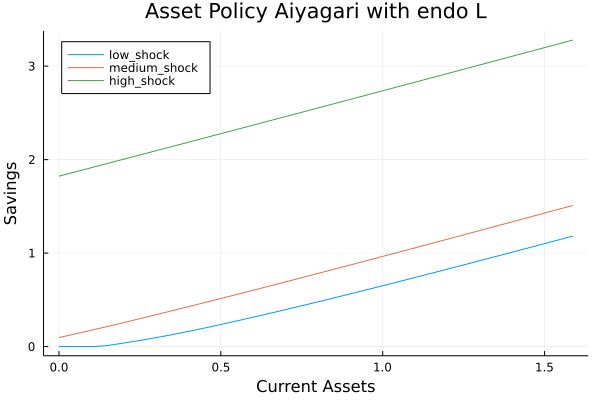
\includegraphics[width=1\textwidth]{endoL_A_p.png} % first figure itself
        \caption{Asset Policy Function}
    \end{minipage}\hfill
    \begin{minipage}{0.45\textwidth}
        \centering
        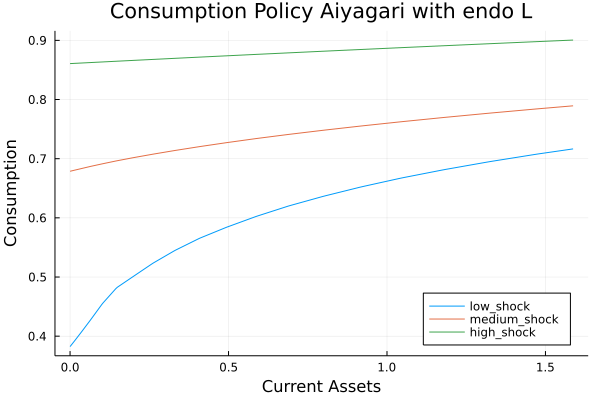
\includegraphics[width=1\textwidth]{endoL_C_p.png} % second figure itself
        \caption{Consumption Policy Function}
    \end{minipage}
\end{figure}

\begin{figure}[h]
    \centering
    \begin{minipage}{0.45\textwidth}
        \centering
        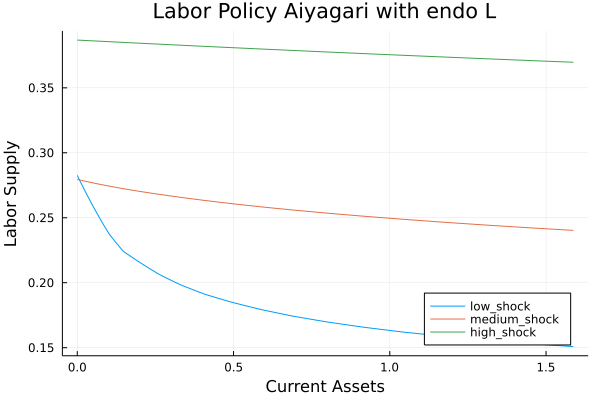
\includegraphics[width=1\textwidth]{endoL_L_p.png} % first figure itself
        \caption{Labor Policy Function}
    \end{minipage}\hfill
    \begin{minipage}{0.45\textwidth}
        \centering
        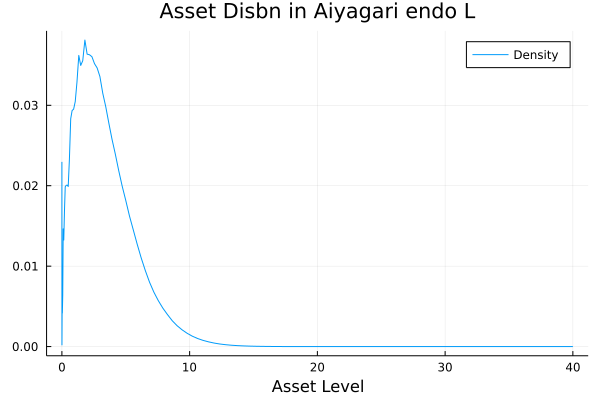
\includegraphics[width=1\textwidth]{endoL_A_dis.png} % second figure itself
        \caption{Asset Distribution}
    \end{minipage}
\end{figure}



\end{document}